\documentclass[11pt,oneside,openany,headings=optiontotoc,11pt,numbers=noenddot]{article}

\usepackage[a4paper]{geometry}
\usepackage[utf8]{inputenc}
\usepackage[T1]{fontenc}
\usepackage{lmodern}
\usepackage[ngerman]{babel}
\usepackage{ngerman}

\usepackage[onehalfspacing]{setspace}

\usepackage{fancyhdr}
\usepackage{fancybox}

\usepackage{rotating}
\usepackage{varwidth}

%Struktogramme
\usepackage[german,curves]{struktex}

\usepackage{pdflscape}
\usepackage{changepage}
\usepackage{graphicx}
\usepackage[bottom]{footmisc}
\usepackage{transparent}
\usepackage{graphbox}
\graphicspath{
	{Pics/PDFs/}
	{Pics/JPGs/}
	{Pics/PNGs/}
}
\usepackage{caption}
\usepackage{wrapfig}
\usepackage{marginnote}
\usepackage{tabularx}
\usepackage{dashrule}
\usepackage{soulutf8}
\usepackage{hhline}
%arydshln suppresses vertical lines in table
%\usepackage{arydshln}
\usepackage{multirow}
\usepackage{enumerate}
\usepackage[hidelinks]{hyperref}
\usepackage{listings}

\usepackage[table]{xcolor}
\usepackage{array}
\usepackage{enumitem,amssymb,amsmath}
\usepackage{interval}
\usepackage{cancel}
\usepackage{stmaryrd}
\usepackage{wasysym}
\usepackage{polynom}
\usepackage{diagbox}
\usepackage{dashrule}
\usepackage{framed}
\usepackage{mdframed}
\usepackage{karnaugh-map}
\usepackage{pdfpages}

\usepackage{blindtext}

\usepackage{eso-pic}

\usepackage{amssymb}
\usepackage{eurosym}

\usepackage[pages=some]{background}
\pagestyle{headings}
\renewcommand{\headrulewidth}{0.2pt}
\renewcommand{\footrulewidth}{0.2pt}
\newcommand*{\underdownarrow}[2]{\ensuremath{\underset{\overset{\Big\downarrow}{#2}}{#1}}}
\setlength{\fboxsep}{5pt}
\newcommand{\explainBelow}[3]{\underbrace{#1}_{\parbox{\widthof{#3}}{\footnotesize\raggedright #2}}}
\newcommand{\explainAbove}[3]{\overbrace{#1}^{\parbox{\widthof{#3}}{\footnotesize\raggedright #2}}}
\newcommand\footnoteref[1]{\protected@xdef\@thefnmark{\ref{#1}}\@footnotemark}


% Codestyle defined
\definecolor{codegreen}{rgb}{0,0.6,0}
\definecolor{codegray}{rgb}{0.5,0.5,0.5}
\definecolor{codepurple}{rgb}{0.58,0,0.82}
\definecolor{backcolour}{rgb}{0.95,0.95,0.92}
\definecolor{deepgreen}{rgb}{0,0.5,0}
\definecolor{darkblue}{rgb}{0,0,0.65}
\definecolor{mauve}{rgb}{0.40, 0.19,0.28}
\colorlet{exceptioncolour}{yellow!50!red}
\colorlet{commandcolour}{blue!60!black}
\colorlet{numpycolour}{blue!60!green}
\colorlet{specmethodcolour}{violet}

%Neue Spaltendefinition
\newcolumntype{L}[1]{>{\raggedright\let\newline\\\arraybackslash\hspace{0pt}}m{#1}}
\newcolumntype{M}{>{\centering\arraybackslash}X}
\newcommand{\cmnt}[1]{\ignorespaces}
%Textausrichtung ändern
\newcommand\tabrotate[1]{\rotatebox{90}{\raggedright#1\hspace{\tabcolsep}}}

%Intervall-Konfig
\intervalconfig {
	soft open fences
}

%Bash
\lstdefinestyle{BashInputStyle}{
	language=bash,
	basicstyle=\small\sffamily,
	backgroundcolor=\color{backcolour},
	columns=fullflexible,
	backgroundcolor=\color{backcolour},
	breaklines=true,
}
%Java
\lstdefinestyle{JavaInputStyle}{
	language=Java,
	backgroundcolor=\color{backcolour},
	aboveskip=1mm,
	belowskip=1mm,
	showstringspaces=false,
	columns=flexible,
	basicstyle={\footnotesize\ttfamily},
	numberstyle={\tiny},
	numbers=none,
	keywordstyle=\color{purple},,
	commentstyle=\color{deepgreen},
	stringstyle=\color{blue},
	emph={out},
	emphstyle=\color{darkblue},
	emph={[2]rand},
	emphstyle=[2]\color{specmethodcolour},
	breaklines=true,
	breakatwhitespace=true,
	tabsize=2,
}
%Python
\lstdefinestyle{PythonInputStyle}{
	language=Python,
	alsoletter={1234567890},
	aboveskip=1ex,
	basicstyle=\footnotesize,
	breaklines=true,
	breakatwhitespace= true,
	backgroundcolor=\color{backcolour},
	commentstyle=\color{red},
	otherkeywords={\ , \}, \{, \&,\|},
	emph={and,break,class,continue,def,yield,del,elif,else,%
		except,exec,finally,for,from,global,if,import,in,%
		lambda,not,or,pass,print,raise,return,try,while,assert},
	emphstyle=\color{exceptioncolour},
	emph={[2]True,False,None,min},
	emphstyle=[2]\color{specmethodcolour},
	emph={[3]object,type,isinstance,copy,deepcopy,zip,enumerate,reversed,list,len,dict,tuple,xrange,append,execfile,real,imag,reduce,str,repr},
	emphstyle=[3]\color{commandcolour},
	emph={[4]ode, fsolve, sqrt, exp, sin, cos, arccos, pi,  array, norm, solve, dot, arange, , isscalar, max, sum, flatten, shape, reshape, find, any, all, abs, plot, linspace, legend, quad, polyval,polyfit, hstack, concatenate,vstack,column_stack,empty,zeros,ones,rand,vander,grid,pcolor,eig,eigs,eigvals,svd,qr,tan,det,logspace,roll,mean,cumsum,cumprod,diff,vectorize,lstsq,cla,eye,xlabel,ylabel,squeeze},
	emphstyle=[4]\color{numpycolour},
	emph={[5]__init__,__add__,__mul__,__div__,__sub__,__call__,__getitem__,__setitem__,__eq__,__ne__,__nonzero__,__rmul__,__radd__,__repr__,__str__,__get__,__truediv__,__pow__,__name__,__future__,__all__},
	emphstyle=[5]\color{specmethodcolour},
	emph={[6]assert,range,yield},
	emphstyle=[6]\color{specmethodcolour}\bfseries,
	emph={[7]Exception,NameError,IndexError,SyntaxError,TypeError,ValueError,OverflowError,ZeroDivisionError,KeyboardInterrupt},
	emphstyle=[7]\color{specmethodcolour}\bfseries,
	emph={[8]taster,send,sendMail,capture,check,noMsg,go,move,switch,humTem,ventilate,buzz},
	emphstyle=[8]\color{blue},
	keywordstyle=\color{blue}\bfseries,
	rulecolor=\color{black!40},
	showstringspaces=false,
	stringstyle=\color{deepgreen}
}

\lstset{literate=%
	{Ö}{{\"O}}1
	{Ä}{{\"A}}1
	{Ü}{{\"U}}1
	{ß}{{\ss}}1
	{ü}{{\"u}}1
	{ä}{{\"a}}1
	{ö}{{\"o}}1
}

% Neue Klassenarbeits-Umgebung
\newenvironment{worksheet}[3]
% Begin-Bereich
{
	\newpage
	\sffamily
	\setcounter{page}{1}
	\ClearShipoutPicture
	\AddToShipoutPicture{
		\put(55,761){{
				\mbox{\parbox{385\unitlength}{\tiny \color{codegray}BBS I Mainz, #1 \newline #2
						\newline #3
					}
				}
			}
		}
		\put(455,761){{
				\mbox{\hspace{0.3cm}
\includegraphics[width=0.2\textwidth]{../../logo.pdf}}
			}
		}
	}
}
% End-Bereich
{
	\clearpage
	\ClearShipoutPicture
}

\setlength{\columnsep}{3em}
\setlength{\columnseprule}{0.5pt}

\geometry{left=1.50cm,right=1.50cm,top=3.00cm,bottom=1.00cm,includeheadfoot}
\pagestyle{plain}
\pagenumbering{arabic}

\begin{document}
	\begin{worksheet}{Informationsverarbeitung}{Lernabschnitt: Betreuen von IT-Systemen}{Datenschutz und Datensicherheit - Maßnahmen zur Datensicherung und - archivierung}
		\section{Datensicherung}
		Unabhängig davon, ob man sich heutzutage im privaten oder aber im beruflichen Bereich bewegt, die Datenflut, die tagtäglich generiert wird ist enorm. Sicher kann dabei zwischen wichtigen und unwichtigen oder relevanten und irrelevanten unterschieden werden. Unabhängig vom betrachteten Bereich ist aber klar: \texttt{Wenn die Daten weg sind, dann ärgern wir uns.}\\
		Um diesem Phänomen entgegenzuwirken, haben wir die Möglichkeit einem eventuellen Datenverlust, durch welche Ursache auch immer, vorzusorgen\footnote{Hierbei ist natürlich zu beachten, dass ein vollkommener Schutz gegen Datenverlust unmöglich ist.} Nachfolgend wollen wir die gängigen Methoden der Datensicherung\footnote{Nachfolgend immer als Backup bezeichnet.} näher beleuchten.
		\subsection*{Bewertungskriterien}
		Bei der Wahl der Backup-Variante gibt es diverse Kriterien, die zu beachten sind.\\
		\par\noindent
		\begin{minipage}{0.48\textwidth}
			\begin{itemize}
				\itemsep0em
				\item Speicherbedarf
				\item Geschwindigkeit (Performance)
				\begin{itemize}
					\itemsep0em
					\item bei der Sicherung
					\item bei der Wiederherstellung
				\end{itemize}
			\end{itemize}
		\end{minipage}
		\hfill
		\begin{minipage}{0.48\textwidth}
			\begin{itemize}
				\item Sicherheit
				\begin{itemize}
					\item bei Ausfall
					\item bei Beschädigung
				\end{itemize}
			\end{itemize}
		\end{minipage}\\
		\subsection{Vollbackup}
		Das Vollbackup bzw. die Vollsicherung kann man salopp als das Beschreiben was so mancher 0815-Computer Nutzer mit seinen Daten zu Hause macht. Bei dieser Variante werden bei jedem Backup alle vorhandenen Daten vom Produktivsystem, unabhängig ihrer Aktualität, kopiert und ohne entsprechende Komprimierung auf dem dafür vorgesehenen Sicherungslaufwerk gespeichert. Das bedeutet, das Backup hat den gleichen Speicherbedarf, wie die zu sichernden Daten.\\
		\par\noindent
		Bei dieser Backup-Variante müssen zur Wiederherstellung nur die Daten vom Sicherungslaufwerk zum entsprechenden Zeitpunkt gewählt und auf das Produktivlaufwerk \grqq{}kopiert\grqq{} werden.\\
		Da hier der komplette Datensatz wiederhergestellt wird entfallen aufwändige Rechenarbeiten, womit die Wiederherstellungszeit entsprechend kurz ist. Die Geschwindigkeit hängt hier lediglich von der Übertragungsrate zwischen den zwei Laufwerken ab.\\
		\par\noindent
		Wie bereits im ersten Absatz angedeutet hat das Vollbackup einen erheblichen Speicherbedarf. Hierbei finden sich die gleichen Dateien mehrfach \grq{}irgendwo\grq{} auf den verschiedenen Laufwerken und nehmen unnötig viel Platz in Anspruch.\\
		\newpage
		\noindent
		Aufgrund des intensiven Speicherbedarfs diese Variante auch sehr kostspielig, da der Speicherplatz beschafft und so zur Verfügung gestellt werden muss.\\
		\par\noindent
		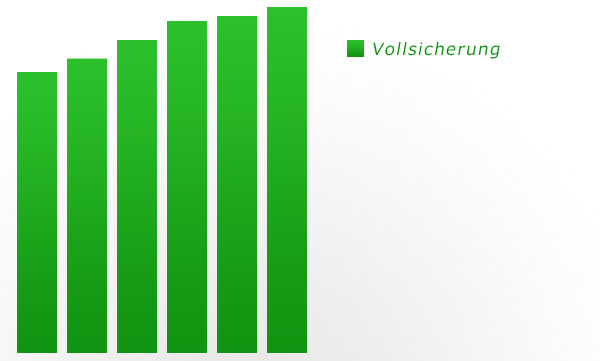
\includegraphics[width=0.98\textwidth]{../99_Bilder/01_voll.jpg}\\
		\tiny{Quelle: \href{https://www.grundlagen-computer.de/backup/backup-strategien-inkrementell-differentiell-und-vollbackup}{Grundlagen Computer Backup Strategien} (05.01.2020)}\\
		\footnotesize{Dieses Schaubild veranschaulicht den Speicherbedarf beim Vollbackup.}\normalsize
		\subsection{Differentielles Backup}
		Grundlage für das differentielle Backup ist ein initial durchgeführtes Vollbackup, auf dem zu jedem Sicherungszeitpunkt aufgebaut wird.\\
		Zu jedem Sicherungszeitpunkt werden bei dieser Variante lediglich die Unterschiede zwischen den aktuellen Daten und dem initialen Vollbackup gesichert. Zu jeder Sicherung werden also alle Dateien des Produktivsystems gesichert, die seit dem initialen Vollbackup verändert wurden oder neu hinzugekommen sind.\\
		\par\noindent
		Bei der Wiederherstellung wird das initiale Vollbackup sowie das differentielle Backup zum gewünschten Zeitpunkt benötigt. Eine entsprechende Rechenarbeit ist aber notwendig, um die beiden Stände zu integrieren und den ursprünglichen Datenzustand wiederherzustellen.\\
		Dennoch benötigt diese Variante aufgrund der Teilsicherung verhältnismäßig wenig Speicherplatz.\\
		\par\noindent
		Obwohl diese Variante pro Sicherungsdurchgang vergleichsweise wenig Speicher benötigt ist der gesamte Speicherbedarf dennoch immens, da im Prinzip jedes vorherige Backup nochmals gespeichert wird.\\
		\par\noindent
		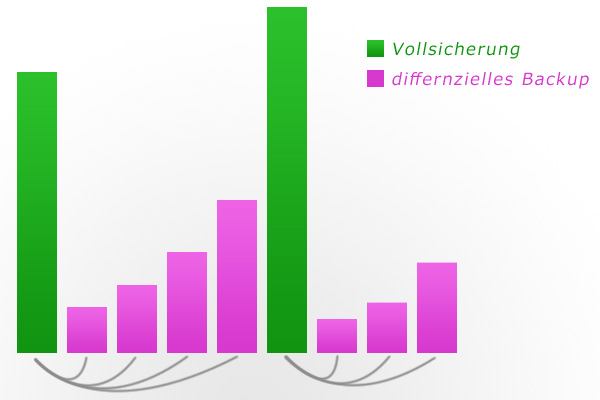
\includegraphics[width=0.98\textwidth]{../99_Bilder/01_diff.jpg}\\
		\tiny{Quelle: \href{https://www.grundlagen-computer.de/backup/backup-strategien-inkrementell-differentiell-und-vollbackup}{Grundlagen Computer}(05.01.2020)}\\
		\footnotesize{Das Schaubild verdeutlicht die nach jedem Sicherungsdurchlauf gesicherten Daten.}\normalsize
		\subsection{Inkrementelles Backup}
		Zuletzt betrachten wir das inkrementelle Backup, welches wie das differentielle Backup, ein initiales Vollbackup benötigt. Zu jedem Sicherungszeitpunkt werden lediglich die Daten gespeichert, die sich seit dem letzten Backup (Teilbackup) verändert haben oder neu hinzugekommen sind.\\
		Diese Methode wird auch als \textit{Forward Delta Verfahren} bezeichnet. Dem gegenüber steht das sogenannte \textit{Reverse Delta Verfahren}, bei dem die Datenunterschiede (Veränderungen bzw. neue Daten) in das bestehende initiale Vollbackup integriert werden.\\
		\par\noindent
		Zur Wiederherstellungen werden entsprechende Kontrolldaten benötigt. Diese dienen dazu, dass die Teilsicherungen an den korrekten Stellen im initialen Vollbackup integriert werden können. Daher ist eine hohe Rechenarbeit nötig, da die einzelnen Teilbackups in das initiale Vollbackup integriert und dadurch der ursprüngliche Datenzustand wiederhergestellt werden müssen.\\
		\par\noindent
		Der Speicherbedarf bei dieser Variante ist sehr gering, da ausschließlich die Differenzen zum vorherigen Backup gespeichert werden. Auf diese Weise kann eine redundante Speicherung von Daten umgangen werden.\\
		Ausschließlich die zuvor erwähnten Kontrolldaten erhöhen den Speicherbedarf um rund 10\%.\\
		\par\noindent
		Das größte Manko dieser Methode ist das aufwändige und teils problematische Wiederherstellen der Daten. Dadurch kann eine entsprechende Wiederherstellung, im Vergleich zum Vollbackup, sehr viel mehr Zeit in Anspruch nehmen.\\
		Zudem ist eine vollständige Wiederherstellung des Datenzustands nicht möglich, sollte auch nur ein Teilbackup geschweige denn das initiale Vollbackup fehlen.\\
		\par\noindent
		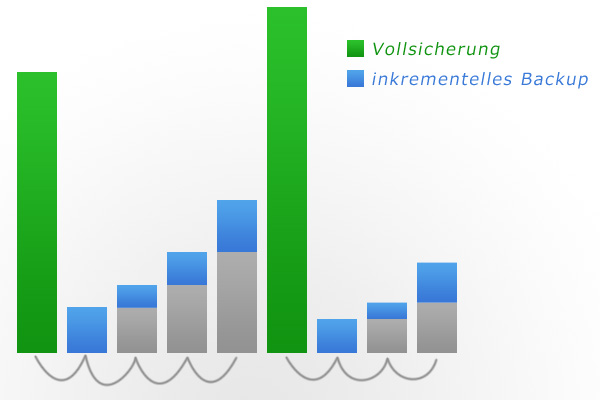
\includegraphics[width=0.98\textwidth]{../99_Bilder/01_ink.jpg}\\
		\tiny{Quelle: \href{https://www.grundlagen-computer.de/backup/backup-strategien-inkrementell-differentiell-und-vollbackup}{Grundlagen Computer}(05.01.2020)}\\
		\footnotesize{Das Schaubild zeigt die zu jedem Sicherungszeitpunkt gespeicherten Datenmengen.}\normalsize
	\end{worksheet}
\end{document}